\documentclass[11pt, letterpaper]{article}   	% use "amsart" instead of "article" for AMSLaTeX format
\usepackage{geometry}                		% See geometry.pdf to learn the layout options. There are lots.
\geometry{letterpaper}                   		% ... or a4paper or a5paper or ... 
%\geometry{landscape}                		% Activate for for rotated page geometry
%\usepackage[parfill]{parskip}    		% Activate to begin paragraphs with an empty line rather than an indent
\usepackage{graphicx}				% Use pdf, png, jpg, or eps§ with pdflatex; use eps in DVI mode
								% TeX will automatically convert eps --> pdf in pdflatex		
\usepackage{amssymb}
\usepackage{amsmath}
%\usepackage{naaclhlt2013}

\usepackage{cite}
\title{Alignment with Minimum Translation Units}
%\author{The Author}
%\date{}							% Activate to display a given date or no date

\begin{document}
\maketitle
\section{Task definition}
A sentence is a sequence of words $S=w_1 w_2 ... w_n $, where $w_i$ is the $i$-th word of the sentence. 
A span is a continuous ordered set $\{i|k\leqslant i \leqslant l\}$ (or equivalently represented as $[i,j]$). 
%A phrase $S_{[i,j]}=w_i...w_j$ is a subsequence of $S$. 
%A segmentation of sentence $S$ is a set of spans $seg=\{p | \bigcup_{p}=[1,n] \wedge \bigcap_{p} = \emptyset\}$.
\iffalse
\begin{equation}
\forall_{1\leqslant i \leqslant |S|} (\exists_{p\in seg} i \in p)  \wedge
\forall_{1\leqslant i \leqslant |S|} \forall_{p,p' \in seg} ({(i \in p \wedge i \in p') \rightarrow p=p'})
\end{equation}
\fi
Given a source sentence $S$ with length $n$ and a target sentence $T$ with length $m$, a phrasal alignment $A$ is a set of span pairs $A=\{(s,t) \, | \, \bigcup_{s} = [1,n], \bigcap_{s} = \emptyset,  \bigcup_{t} = [1,m], \bigcap_{t} = \emptyset \}$. Our task is to 
\begin{itemize} 
\item define a model $f: \{S,T,A\} \rightarrow \mathbf{R}$
\item estimate the parameters in $f$
\item given $S,T$, use some algorithm to find $A=\operatorname*{argmax}_{A} f(S,T,A)$.
\end{itemize}
 
\section{Notation related to phrase}

\begin{itemize}
%\item Word content: In the above definition, $w_i$ not only contains the word content but also the position information. For convenience, we denote $c(w_i)$ as the content of the word $w_i$. For example, in sentence ``tweet a tweet'' where the word ``tweet'' appears in positions $1$ and $3$, we say $w_1 < w_3$ and $c(w_1) = c(w_3)$.

\item Phrase: Given a span $s=[i,j]$, the phrase corresponding to  that span is $S_s=w_i w_{i+1}...w_j$

\item Span boundary: Given a span $s=[i,j]$, we define its left boundary position as $left(s)=i$, right boundary position as $right(s)=j$. 

\item Span pair: We define span pair $spair=(s,t)$, source span $src(spair)=s$, target span $tgt(spair)=t$.

\item Segmentation of span: $seg(s)=\{s'| \bigcup s' = s, \bigcap s' = \emptyset\}$
\end{itemize}

\section{Model $f$} 
We can define various model $f$. Here we give some examples.
\begin{itemize}

\item Model 1:
\begin{enumerate}
\item generate a group of phrase pairs $\{(ps,pt)\}$
\item order the phrase pairs into sentence pairs
\end{enumerate}

The probability of tuple $(S,T,A)$ is 
\begin{equation} \label{eq:obj1}
p(S,T,A)=\prod_{(s,t)\in A}p(S_s,T_t)
\end{equation}

\item Model 1C:
same as Model 1, except that we adopt conditional probability for phrase pair. $p(S_s,T_t)=p(T_t|S_s)*p(S_s)$ and $p(S_s)=\prod p(w|w\in S_s)$.

\item Model 2:

\begin{enumerate}
\item generate begin of sentence pair $(``<s>'',``<s>'')$
\item generate phrase pair $(ps,pt)$, append $ps$ to the end of generated partial source sentence
\item repeat step 2 step until end of sentence pairs $(``</s>'',``</s>'')$ was generated.
\item order the target phrases generated in step 2 into target sentence
\end{enumerate}

Let's assume the reordering follow a uniform distribution.
The probability of tuple $(S,T,A)$ is 
\begin{equation} \label{eq:obj2}
p(S,T,A))=\prod_{(s_i,t_i) \in A} p((S_{s_i},T_{t_i})| (S_{s_{i-1}},T_{t_{i-1}}) ... (S_{s_{1}},T_{t_{1}}))
\end{equation}
where $left(s_i)- right(s_{i-1})=1$

\item Model 3:
Same as model 2, but here we assume the reordering follow a slightly more complicated distribution than uniform.
\begin{equation} \label{eq:obj3}
f(S,T,A))=\prod_{(s_i,t_i) \in A} p((S_{s_i},T_{t_i})| (S_{s_{i-1}},T_{t_{i-1}}) ... (S_{s_{1}},T_{t_{1}})) p(d(i) | d(i-1) ... d(1)) )
\end{equation}
where $left(s_i)- right(s_{i-1})=1$, \quad $d(i)=left(t_i)- right(t_{i-1})$
\end{itemize}

\section{Parameter estimation}
\subsection{Basic Approach}
Given a sentence pair $(S,T)$, $p(S,T)=\sum_{A}p(S,T,A)$.\\
Given a parallel corpus $C$ where $A$ is the latent data, 
\begin{equation}p(C)=\prod_{(S,T) \in C} p(S,T)=\prod_{(S,T) \in C} \sum_{A} p(S,T,A) \end{equation}
We estimate the parameters by optimizing the objective function $p(C)$. EM is one of the ways to do the optimization with latent variables.

\subsection{Complexity}
Given a source sentence $S$ with length $n$, then we have number of phrases $\frac{n^2+n}{2}$ and number of segmentations $\sum\limits_{i=1}^n {n \choose i} = 2^n$. 

Given a source sentence $S$ with length $n$ and a target sentence $T$ with length $m$.  Let $n \leqslant m $, the number of possible phrasal alignments 
\begin{equation}
|\{A\}|= \sum \limits_{i=1}^n {n \choose i}{m \choose i}i!  > \sum \limits_{i=1}^n {n \choose i}{n \choose i} = {2n \choose n} \sim \frac{4^n}{n^{1/2} \sqrt{\pi}}.
\end{equation}

Search for the best phrasal alignment is NP-Hard, sum over all alignments is PSPACE-hard \cite{denero-acl-08}.

%If the phrase segmentation of the source sentence is given, then this problem can be reduced to the longest path problem which is NP-complete.  So the original problem is NP-hard. 

\subsection{Pruning}
It's impractical to do parameter estimation and search in the original model space. Below are some heuristic ways to do pruning.
\begin{itemize}
\item filter out phrases appearing less than 5 times in the corpus, but keep all unigrams \cite{marcu-wong-02}
\item filter out phrases which is not compatible with word alignments. \cite{denero-06-wmt}
\end{itemize}

\subsection{Search Algorithm}
\begin{itemize}
\item Greedily hill climbing, with some heuristic actions : breaking and merging concepts, swapping words between concepts, and moving words across concept. \cite{marcu-wong-02}
\item Exponential-time dynamic programming with word alignment constraint.  \cite{denero-06-wmt}
\end{itemize}

\section{Analysis}
Why both of them underperform heuristic phrase extraction from word alignment?

\cite{marcu-wong-02} why?

\cite{denero-06-wmt} did not generate new phrases.

My guess is for MT, the decoding algorithm and LM are so powerful that the probability of phrase pair doesn't matter a lot. And the content of phrase pairs matter more. The phrasal alignment approaches don't necessarily generate more correct phrase pairs than the heuristic way.

\subsection{Pilot experiment}
If the guess above is correct, then the contribution from EM will not be significant. Initialization will be good enough. To test it, we just use the phrase table estimated from the initialization step for decoding. And compare the performance with state-of-the-art phrase table extraction. 

\subsubsection{Setting}
\begin{itemize}
\item Training Data: corev5
\item Dev Data: corev5.6 tune
\item Test Data: corev5.6 test
\item Language model: trigram language model trained on GIGAWORD3.
\item System: Moses \cite{moses-07}
\end{itemize}

\subsubsection{Phrase pairs extraction approaches}
We try and compare following different approaches.

\begin{enumerate}
\item Approach in \cite{marcu-wong-02}. Filter out phrases appearing less than 5 times in the corpus, but keep all unigrams, attach t-distribution score to them.

\item Use Model 1C with constraint 0 $<$ phrase length $<$ X, attach IBM model 1 score for each phrase pair. How to choose the X? State-of-the-art MT system Moses\cite{moses-07} sets the maximal phrase length to be 7. We can try different value from 5 to 7.

\item State-of-the-art heuristic phrase extraction: run GIZA++($1^52^5H^53^34^3$), compute the viterbi alignment for source-to-target and target-to-source directions, use heuristic grow-diag-final to combine the two alignments. Extract the phrases according to the alignment constraint. For each phrase pair, compute phrasal and lexical conditional probabilities for source-to-target and target-to-source directions.
\end{enumerate}

\subsubsection{Results}
For the Approach in \cite{marcu-wong-02},
Questions: 1. how many phrases will appear more than 5/X times? And what's the average length of such phrases?  

\begin{table}
\centering
\begin{tabular}{ c | c | c | c | c }
 & \multicolumn{2}{c}{\bf{Chinese}} & \multicolumn{2}{|c}{\bf{English}}  \\
  \cline{2-5} 
  \bf{cutoff} & \bf{\#phrases} & \bf{avg. length} & \bf{\#phrases} & \bf{avg. length} \\
  \hline
  1 & 5.07e+07  & 6.40 & 6.57e+07 & 6.69  \\
  \hline
  2 & 5.42e+06 & 5.07 &5.78e+06 & 5.02\\
  \hline
  3 & 1.86e+06  & 4.11 & 2.31e+06& 4.30\\
  \hline
  4 & 1.04e+06 & 3.58 &1.36e+06 &3.86\\
 \hline
  5 & 0.72e+06 & 3.31 & 0.97e+06&3.65\\
 \end{tabular}
 \caption{cutoff frequency vs phrase table size}
  \label{tab:phrase-cutoff}
\end{table}

\begin{figure}[p]
\centering
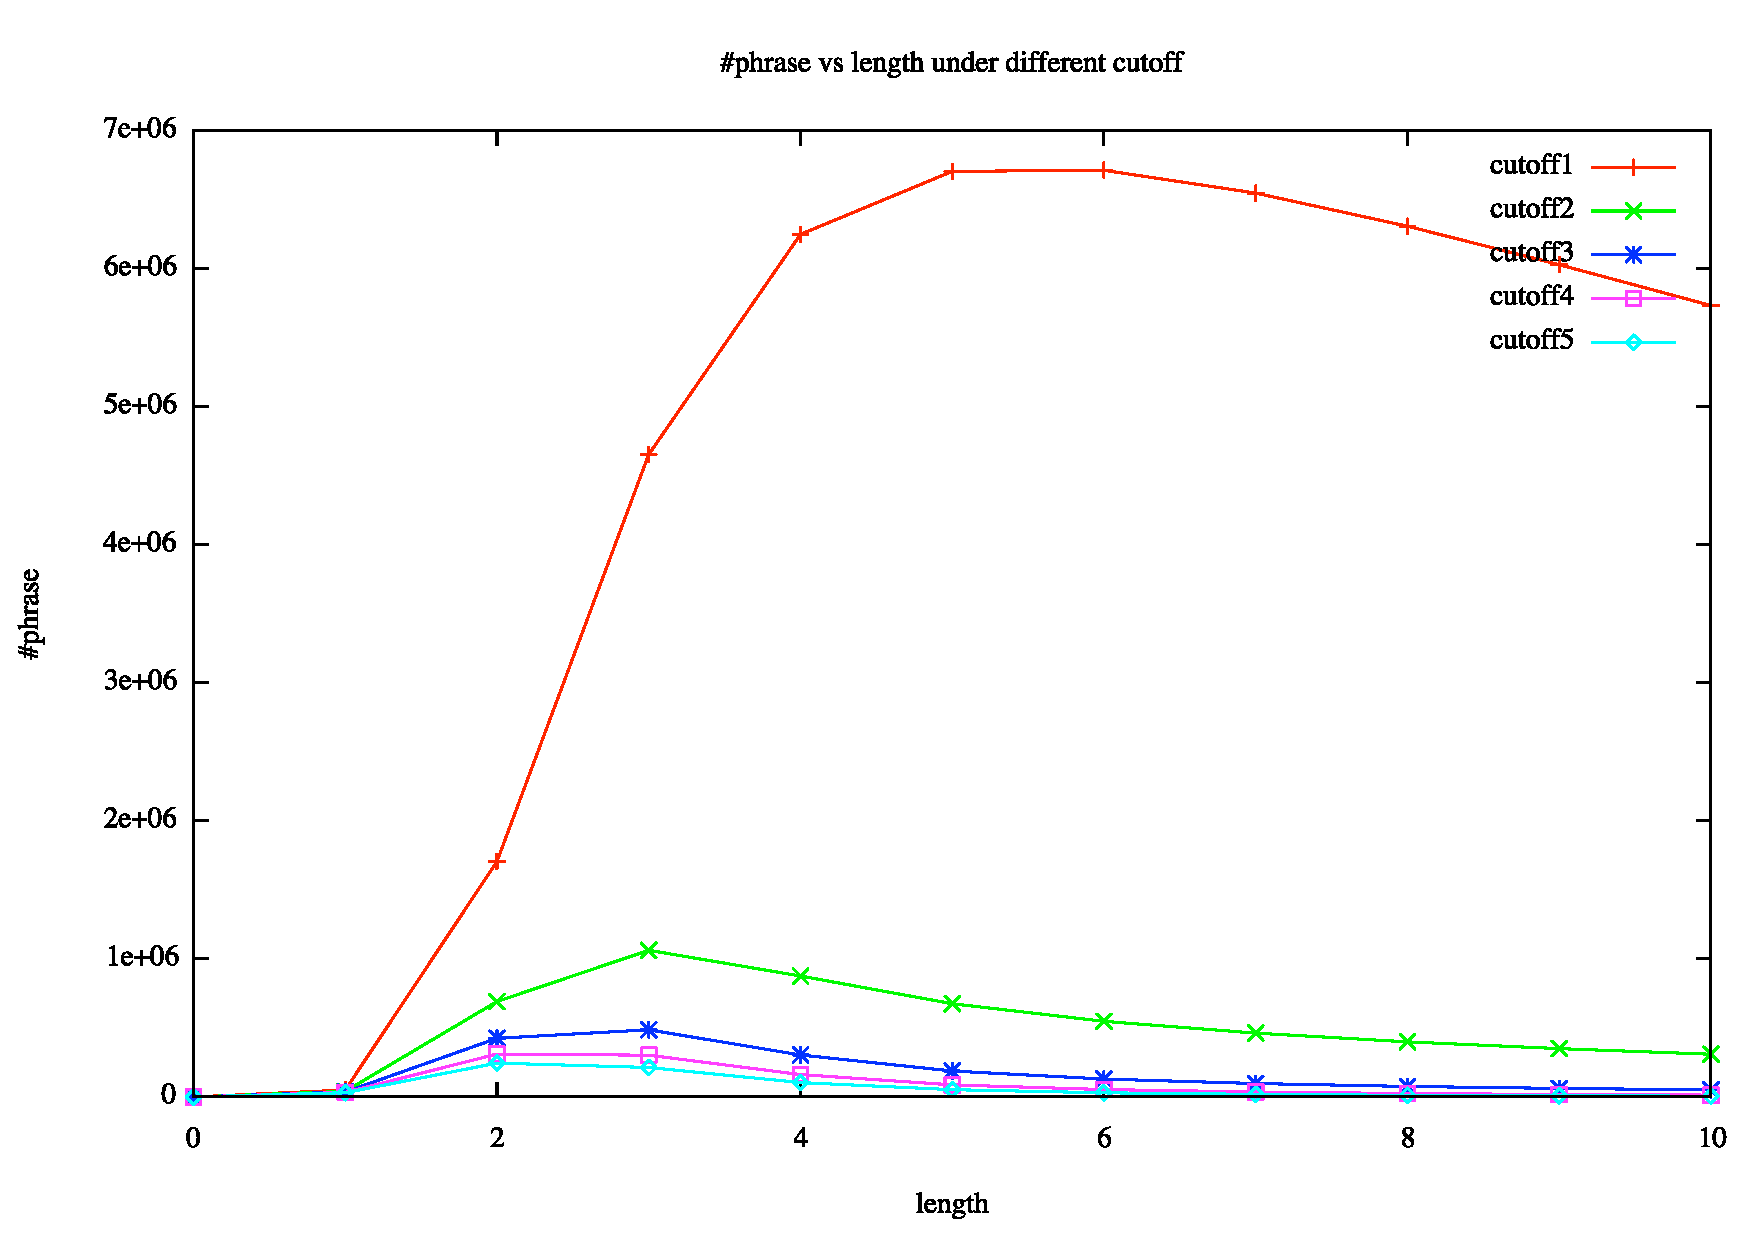
\includegraphics[width=1.0\textwidth]{phrase-count-chinese.pdf}
\caption{phrase count vs cutoff: Chinese}
\label{fig:phrase-count-chinese}
\end{figure}

\begin{figure}[p]
\centering
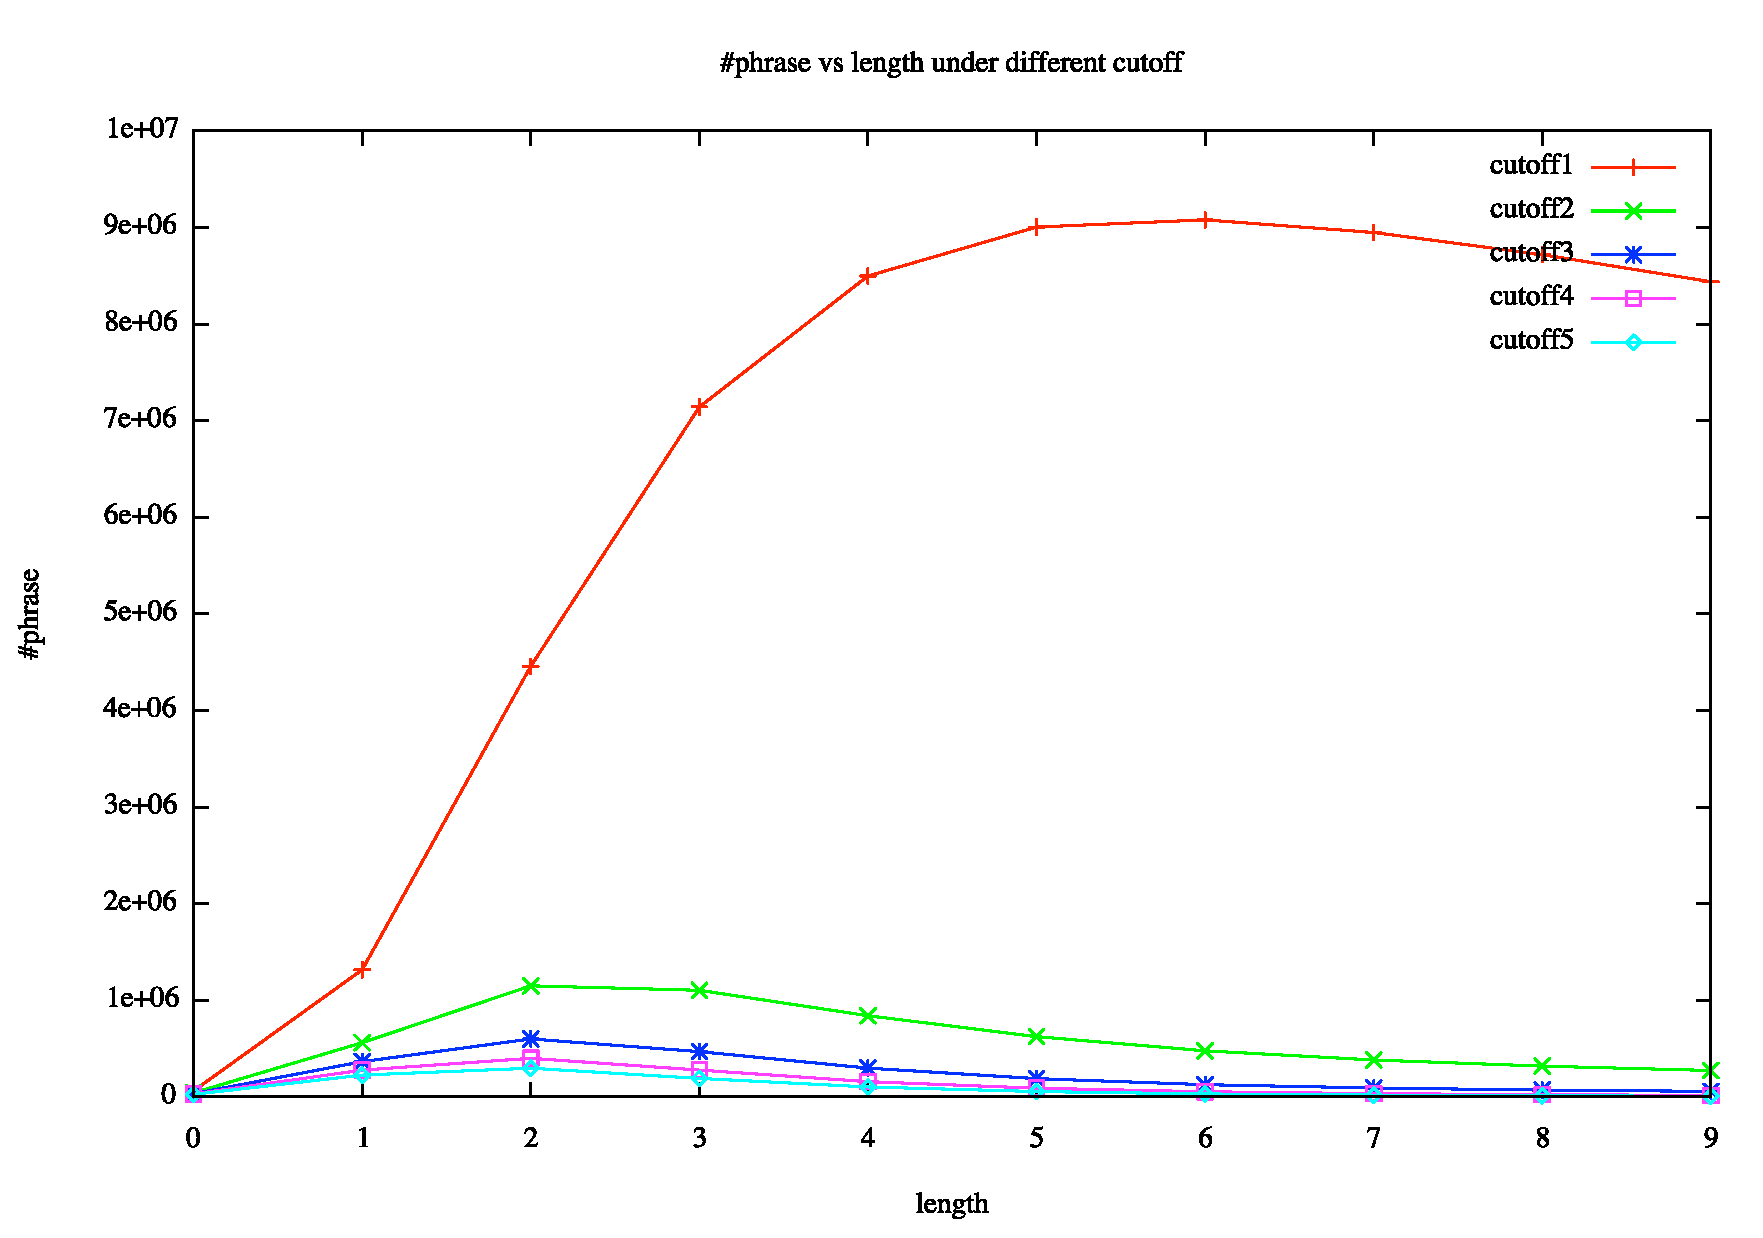
\includegraphics[width=1.0\textwidth]{phrase-count-english.pdf}
\caption{phrase count vs cutoff: English}
\label{fig:phrase-count-english}
\end{figure}

Problem encounter: since I just change to c++11 and gcc 4.8.1. Code compiled on mac, doesn't compile on hpc. 

For State-of-the-art heuristic phrase extraction, 
\begin{enumerate}
\item try blocking the phrase conditional probability.
blocked vs unblocked
BLEU
\end{enumerate}
Problem encounter: meet script offers some options to set value range for any feature. I set the value range for phrase conditional probability to [0,0]. However, the final value generated by meet is not 0.

\bibliography{mybib}
\bibliographystyle{plain}
\end{document}  
